\documentclass[runningheads]{llncs}

% correct bad hyphenation here
\hyphenation{}

%\usepackage{natbib}
\usepackage{url}

% *** MATHS PACKAGES ***
%
\usepackage[cmex10]{amsmath}
\usepackage{amssymb}
\usepackage{stmaryrd}
%\usepackage{amsthm}

% *** ALIGNMENT PACKAGES ***
%
\usepackage{array}
\usepackage{float}  %% Try to improve placement of figures.  Doesn't work well with subcaption package.
\usepackage{subcaption}
\usepackage{caption}

\usepackage{subfiles}
\usepackage{geometry}
\usepackage{listings}
\usepackage[dvipsnames]{xcolor}
\usepackage{verbatim}
\usepackage{listings}% http://ctan.org/pkg/listings
\lstset{
  basicstyle=\ttfamily,
  mathescape
}
\usepackage{alltt}
\usepackage{paralist}

\usepackage{todonotes}
%\usepackage[disable]{todonotes}

% This has to go at the end of the packages.
\usepackage[colorlinks=true,linkcolor=MidnightBlue,citecolor=ForestGreen,urlcolor=Plum]{hyperref}

% Stuff for splitting figures over page breaks
%\DeclareCaptionLabelFormat{continued}{#1~#2 (Continued)}
%\captionsetup[ContinuedFloat]{labelformat=continued}

% *** MACROS ***

\newcommand\agdaRepo{https://github.com/omelkonian/formal-utxo/tree/ed72}

\newcommand{\todochak}[1]{\todo[inline,color=purple!40,author=chak]{#1}}
\newcommand{\todompj}[1]{\todo[inline,color=yellow!40,author=Michael]{#1}}
\newcommand{\todokwxm}[1]{\todo[inline,color=blue!20,author=kwxm]{#1}}
\newcommand{\todojm}[1]{\todo[inline,color=purple!40,author=Jann]{#1}}

\newcommand{\red}[1]{\textcolor{red}{#1}}
\newcommand{\redfootnote}[1]{\red{\footnote{\red{#1}}}}
\newcommand{\blue}[1]{\textcolor{blue}{#1}}
\newcommand{\bluefootnote}[1]{\blue{\footnote{\blue{#1}}}}

%% A version of ^{\prime} for use in text mode
\makeatletter
\DeclareTextCommand{\textprime}{\encodingdefault}{%
  \mbox{$\m@th'\kern-\scriptspace$}%
}
\makeatother

\newcommand{\code}{\texttt}
\renewcommand{\i}{\textit}  % Just to speed up typing: replace these in the final version
\renewcommand{\t}{\texttt}  % Just to speed up typing: replace these in the final version
\newcommand{\s}{\textsf}  % Just to speed up typing: replace these in the final version
\newcommand{\msf}[1]{\ensuremath{\mathsf{#1}}}
\newcommand{\mi}[1]{\ensuremath{\mathit{#1}}}

%% A figure with rules above and below.
\newcommand\rfskip{3pt}
%\newenvironment{ruledfigure}[1]{\begin{figure}[#1]\hrule\vspace{\rfskip}}{\vspace{\rfskip}\hrule\end{figure}}
\newenvironment{ruledfigure}[1]{\begin{figure}[#1]}{\end{figure}}

%% Various text macros
\newcommand{\true}{\textsf{true}}
\newcommand{\false}{\textsf{false}}

\newcommand{\hash}[1]{\ensuremath{#1^{\#}}}

\newcommand\mapsTo{\ensuremath{\mapsto}}
\newcommand\cL{\ensuremath{\{}}
\newcommand\cR{\ensuremath{\}}}

\newcommand{\List}[1]{\ensuremath{\s{List}[#1]}}
\newcommand{\Set}[1]{\ensuremath{\s{Set}[#1]}}
\newcommand{\FinSet}[1]{\ensuremath{\s{FinSet}[#1]}}
\newcommand{\Interval}[1]{\ensuremath{\s{Interval}[#1]}}
\newcommand{\FinSup}[2]{\ensuremath{\s{FinSup}[#1,\linebreak[0]#2]}}
% ^ \linebeak is to avoid a bad line break when we talk about finite
% maps.  We may be able to remove it in the final version.
\newcommand{\supp}{\msf{supp}}

\newcommand{\FPScript}{\ensuremath{\s{Script}}}
\newcommand{\Script}{\FPScript}
\newcommand{\scriptAddr}{\msf{scriptAddr}}
\newcommand{\ctx}{\ensuremath{\s{Context}}}
\newcommand{\toData}{\ensuremath{\s{toData}}}
\newcommand{\fromData}{\msf{fromData}}

\newcommand{\verify}{\msf{verify}}

\newcommand{\mkContext}{\ensuremath{\s{mkContext}}}

\newcommand{\applyScript}[1]{\ensuremath{\llbracket#1\rrbracket}}

% Macros for eutxo things.
\newcommand{\tx}{\mi{tx}}
\newcommand{\TxId}{\ensuremath{\s{TxId}}}
\newcommand{\txId}{\msf{txId}}
\newcommand{\txrefid}{\mi{id}}
\newcommand{\Address}{\ensuremath{\s{Address}}}
\newcommand{\DataHash}{\ensuremath{\s{DataHash}}}
\newcommand{\hashData}{\msf{dataHash}}
\newcommand{\idx}{\mi{index}}
\newcommand{\inputs}{\mi{inputs}}
\newcommand{\outputs}{\mi{outputs}}
\newcommand{\validityInterval}{\mi{validityInterval}}
\newcommand{\scripts}{\mi{scripts}}
\newcommand{\forge}{\mi{forge}}
\newcommand{\sigs}{\mi{sigs}}
\newcommand{\fee}{\mi{fee}}
\newcommand{\addr}{\mi{addr}}
\newcommand{\pubkey}{\mi{pubkey}}
\newcommand{\val}{\mi{value}}  %% \value is already defined

\newcommand{\validator}{\mi{validator}}
\newcommand{\redeemer}{\mi{redeemer}}
\newcommand{\datum}{\mi{datum}}
\newcommand{\datumHash}{\mi{datumHash}}
\newcommand{\datumWits}{\mi{datumWitnesses}}
\newcommand{\Data}{\ensuremath{\s{Data}}}
\newcommand{\Input}{\ensuremath{\s{Input}}}
\newcommand{\Output}{\ensuremath{\s{Output}}}
\newcommand{\OutputRef}{\ensuremath{\s{OutputRef}}}
\newcommand{\Signature}{\ensuremath{\s{Signature}}}
\newcommand{\Ledger}{\ensuremath{\s{Ledger}}}

\newcommand{\outputref}{\mi{outputRef}}
\newcommand{\txin}{\mi{in}}
\newcommand{\id}{\mi{id}}
\newcommand{\lookupTx}{\msf{lookupTx}}
\newcommand{\getSpent}{\msf{getSpentOutput}}

\newcommand{\consumes}[1]{\msf{consumes(#1)}}
\newcommand{\consumesOne}[1]{\msf{consumesOne(#1)}}
\newcommand{\cid}{\mi{cid}}
\newcommand{\inputValue}{\mi{inputValue}}
\newcommand{\rMin}{r_{\mi{min}}}
\newcommand{\rMax}{r_{\mi{max}}}

\newcommand{\Tick}{\ensuremath{\s{Tick}}}
\newcommand{\currentTick}{\msf{currentTick}}
\newcommand{\spent}{\msf{spentOutputs}}
\newcommand{\unspent}{\msf{unspentOutputs}}
\newcommand{\txunspent}{\msf{unspentTxOutputs}}
\newcommand{\utxotx}{\msf{Tx}}

\newcommand{\Quantity}{\ensuremath{\s{Quantity}}}
\newcommand{\Asset}{\ensuremath{\s{Asset}}}
\newcommand{\Policy}{\ensuremath{\s{PolicyID}}}
\newcommand{\Quantities}{\ensuremath{\s{Quantities}}}
\newcommand{\nativeCur}{\ensuremath{\mathrm{nativeC}}}
\newcommand{\nativeTok}{\ensuremath{\mathrm{nativeT}}}

\newcommand{\PublicKey}{\ensuremath{\s{PubKey}}}
\newcommand{\PrivateKey}{\ensuremath{\s{PrivateKey}}}

\newcommand{\pkey}{\ensuremath{\pi_{\mathsf{p}}}}
\newcommand{\skey}{\ensuremath{\pi_{\mathsf{s}}}}

\newcommand\B{\ensuremath{\mathbb{B}}}
\newcommand\N{\ensuremath{\mathbb{N}}}
\newcommand\Z{\ensuremath{\mathbb{Z}}}
\renewcommand\H{\ensuremath{\mathbb{H}}}
%% \H is usually the Hungarian double acute accent
\newcommand{\emptyBs}{\ensuremath{\emptyset}}

\newcommand{\emptymap}{\ensuremath{\{\}}}

\usepackage{etoolbox}

% For anonymisation
\newtoggle{anonymous}
\toggletrue{anonymous}
\iftoggle{anonymous}{
  \newcommand{\Cardano}{CHAIN}
  \newcommand{\Plutus}{LANG}
}{
  \newcommand{\Cardano}{Cardano}
  \newcommand{\Plutus}{Plutus Core}
}

% Names, for consistency
\newcommand{\UTXO}{UTXO}
\newcommand{\UTXOma}{UTXO$_{\textsf{ma}}$}
\newcommand{\EUTXO}{E\UTXO{}}
\newcommand{\ExUTXO}{Extended \UTXO{}}
\newcommand{\CEM}{CEM}

% relaxed float placement
\renewcommand{\topfraction}{.95}
\renewcommand{\bottomfraction}{.7}
\renewcommand{\textfraction}{.15}
\renewcommand{\floatpagefraction}{.66}
\renewcommand{\dbltopfraction}{.66}
\renewcommand{\dblfloatpagefraction}{.66}
\setcounter{topnumber}{9}
\setcounter{bottomnumber}{9}
\setcounter{totalnumber}{20}
\setcounter{dbltopnumber}{9}

%% ------------- Start of document ------------- %%

\begin{document}

\lstset{
  basicstyle=\ttfamily,
  columns=fullflexible,
  keepspaces=true,
}

\title{\UTXOma: \UTXO\ with Multi-Asset Support}
%\title{\UTXOma: \UTXO\ with Multi-Asset Support\\ --- DRAFT --- DRAFT ---}

% First names are abbreviated in the running head.
% If there are more than two authors, 'et al.' is used.

\author{
  Manuel M.T. Chakravarty\inst{1}
  \and
  James Chapman\inst{1}
  \and
  Kenneth MacKenzie\inst{1}
  \and
  Orestis Melkonian\inst{1,2}
  \and
  Jann M\"uller\inst{1}
  \and
  Michael Peyton Jones\inst{1}
  \and
  Polina Vinogradova\inst{1}
  \and
  Philip Wadler\inst{1,2}
  \and
  Joachim Zahnentferner\inst{3}
}

\authorrunning{Chakravarty et al.}
%\authorrunning{--- DRAFT --- DRAFT --- DRAFT ---}

\institute{
  IOHK,
  \email{firstname.lastname@iohk.io}
  \and
  University of Edinburgh,
  \email{orestis.melkonian@ed.ac.uk, wadler@inf.ed.ac.uk}
  \and
  \email{chimeric.ledgers@protonmail.com}
}

\maketitle

\begin{abstract}
A prominent use case of Ethereum smart contracts is the creation of a wide range of \emph{user-defined tokens} or \emph{assets} by way of smart contracts. User-defined assets are \emph{non-native} on Ethereum; i.e., they are not directly supported by the ledger, but require repetitive custom code. This makes them unnecessarily inefficient, expensive, and complex. It also makes them insecure as numerous incidents on Ethereum have demonstrated. Even without stateful smart contracts, the lack of perfect fungibility of Bitcoin assets allows for implementing user-defined tokens as layer-two solutions, which also adds
an additional layer of complexity.

In this paper, we explore an alternative design based on Bitcoin-style \UTXO\ ledgers. Instead of introducing general scripting capabilities together with the associated security risks, we propose an extension of the \UTXO\ model, where we replace the accounting structure of a single cryptocurrency with a new structure that manages an unbounded number of user-defined, native tokens, which we call \emph{token bundles.} Token creation is controlled by \emph{forging policy scripts} that, just like Bitcoin validator scripts, use a small domain-specific language with bounded computational expressiveness, thus favouring Bitcoin's security and computational austerity. The resulting approach is lightweight, i.e., custom asset creation and transfer is cheap, and it avoids use of any global state in the form of an asset registry or similar.

The proposed \UTXOma\ model and the semantics of the scripting language have been formalised in the Agda proof assistant.
\end{abstract}

\keywords{blockchain \and \UTXO{} \and native tokens \and functional programming.}

\section{Introduction}

Bitcoin, the most widely known and most valuable cryptocurrency, uses
a graph-based ledger model built on the concept of \emph{\UTXO{}s} (\emph{unspent
  transaction outputs})~\cite{formal-model-of-bitcoin-transactions,Zahnentferner18-UTxO}. Individual \emph{transactions} consist of a list of \emph{inputs} and a list of \emph{outputs}, where outputs represent a specific \emph{value} (of a cryptocurrency) that is available to be spent by inputs of subsequent transactions. Each output can be spent by (i.e., connect to) exactly one input. Moreover, we don't admit cycles in these connections, and hence we can regard a collection of transactions spending from each other as a directed acyclic graph, where a transaction with $m$ inputs and $n$ outputs is represented by a node in the graph with $m$ edges in and $n$ edges out.
The sum of the values consumed by a transaction's inputs must equal the sum of the values provided by its outputs, thus value is conserved.

Whether an output can be consumed by an input is determined by a function $\nu$ attached to the output, which we call the output's \emph{validator}. A transaction input proves its eligibility to spent an output by providing a \emph{redeemer} value $\rho$, such that \(\nu(\rho) = \true\) --- redeemers are often called \emph{witnesses} in Bitcoin. In the simplest case, the redeemer is a cryptographic hash of the spending transaction signed by an authorised spender's private key, which is checked by the validator, which embeds the corresponding public key. More sophisticated protocols are possible by using more complex validator functions and redeemers --- see \cite{bitml} for a high-level model of what is possible with the functionality provided by Bitcoin.

The benefit of this graph-based approach to a cryptocurrency ledger is that it plays well with the concurrent and distributed nature of blockchains. In particular, it forgoes any notion of shared mutable state, which is known to lead to highly complex semantics in the face of concurrent and distributed computations involving that shared mutable state.

Nevertheless, the \UTXO{} model, generally, and Bitcoin, specifically, has been criticised for the limited expressiveness of programmability achieved by the validator concept. In particular, Ethereum's \emph{account-based ledger} and the associated notion of \emph{contract accounts} has been motivated by the desire to overcome those limitations. Unfortunately, it does so by introducing a notion of shared mutable state, which significantly complicates the semantics of contract code. In particular, contract authors need to understand the subtleties of this semantics or risk introducing security issues (such as the vulnerability to recursive contract invocations that led to the infamous DAO attack~\cite{DAO-attack}).

\paragraph{Contributions.}

The contribution of the present paper is to propose an extension to the basic \UTXO{} ledger model, which
\begin{inparaenum}[(a)]
\item provably increases expressiveness, while simultaneously
\item preserving the dataflow properties of the \UTXO{} graph; in particular, it forgoes introducing any notion of shared mutable state.
\end{inparaenum}
More specifically, we make the following contributions:
%
\begin{itemize}
\item We propose the \emph{\EUTXO{} model}, informally in Section~\ref{sec:informal-eutxo} and formally in Section~\ref{sec:formal-model}.
\item We demonstrate that the \EUTXO{} model supports the implementation of a specific form of state machines (\emph{Constraint Emitting Machines}, or \CEM{}s), which the basic \UTXO{} model does not support, in Section~\ref{sec:expressiveness}.
\item We provide a formalisation of both the \EUTXO{} model
  and Constraint Emitting Machines. We prove a weak bisimulation
  between the two using the Agda proof
  assistant\site{https://github.com/\GitUser/formal-utxo/tree/\AgdaCommit}, building on
  previous work by Melkonian et al.~\cite{formal-eutxo}.
\end{itemize}

Section~\ref{sec:related} summarises related work.

The \EUTXO{} model will be used in the ledger of \Cardano{}, a major blockchain
system currently being developed by IOHK.
It also provides the foundation of Cardano's smart contract platform
\emph{Plutus}\site{https://github.com/input-output-hk/plutus}, which includes a small
functional programming language \emph{\Plutus{}} which is used to implement \script{}s.
Although a technical description of Cardano itself is beyond the scope of this paper,
one can try out the Plutus Platform in an online playground.\site{https://prod.playground.plutus.iohkdev.io/}

Other future work includes a formal comparison of \EUTXO{} with Ethereum's account-based model.

\iftoggle{anonymous}{
\paragraph{Anonymisation.}

For the purposes of submission, we have anonymised the following names:
\begin{itemize}
\item \Cardano{}: a major blockchain system.
\item \Plutus{}: a small functional programming language.
\end{itemize}
}{}

\section{Multi-Asset Support}
\label{sec:multicurrency}

In Bitcoin's ledger model~\cite{Nakamoto,formal-model-of-bitcoin-transactions,Zahnentferner18-UTxO}, transactions spend as yet \emph{unspent transaction outputs \textup{(}\!\UTXO{}s\textup{)}}, while supplying new unspent outputs to be consumed by subsequent transactions.
Each individual \UTXO\ locks a specific \emph{quantity} of cryptocurrency by imposing specific conditions that need to be met to spend that quantity, such as for example signing the spending transaction with a specific secret cryptographic key, or passing some more sophisticated conditions enforced by a \emph{validator script}.
Quantities of cryptocurrency in a transaction output are represented as an integral number of the smallest unit of that particular cryptocurrency --- in Bitcoin, these are Satoshis.
To natively support multiple currencies in transaction outputs, we generalise those integral quantities to natively support the dynamic creation of new user-defined \emph{assets} or \emph{tokens}. Moreover, we require a means to forge tokens in a manner controlled by an asset's \emph{forging policy}.

We achieve all this by the following three extensions to the basic \UTXO\ ledger model that are further detailed in
the remainder of this section.
%
\begin{enumerate}
\item Transaction outputs lock a \emph{heterogeneous token bundle} instead of only an integral value of one cryptocurrency.
\item We extend transactions with a \emph{forge} field. This is a token bundle of tokens that are created (minted) or destroyed (burned) by that transaction.
\item We introduce \emph{forging policy scripts \textup{(}FPS\textup{)}} that govern the creation and destruction of assets in forge fields. These scripts are not unlike the validators locking outputs in \UTXO.
\end{enumerate}

\subsection{Token bundles}

We can regard transaction outputs in an \UTXO\ ledger as pairs \((\val, \nu)\) consisting of a locked value $\val$ and a validator script $\nu$ that encodes the spending condition. The latter may be proof of ownership by way of signing the spending transaction with a specific secret cryptography key or a temporal condition that allows an output to be spent only when the blockchain has reached a certain height (i.e. a certain number of blocks have been produced).

To conveniently use multiple currencies in transaction outputs, we want each output to be able to lock varying quantities of multiple different currencies at once in its $\val$ field.
This suggests using finite maps from some kind of \emph{asset identifier} to an integral quantity as a concrete representation, e.g. $\texttt{Coin} \mapsto 21$.
Looking at the standard \UTXO\ ledger rules~\cite{Zahnentferner18-UTxO}, it becomes apparent that cryptocurrency quantities need to be monoids.
It is a little tricky to make finite maps into a monoid, but the solution is to think of them as \emph{finitely supported functions} (see Section~\ref{sec:fsfs} for details).

If want to use \emph{finitely supported functions} to achieve a uniform
representation that can handle groups of related, but \emph{non-fungible} tokens, we need to go a step further.
In order to not lose the grouping of related non-fungible tokens (all house tokens issued by a specific entity, for example) though, we need to move to a two-level structure --- i.e., finitely-supported functions of finitely-supported functions. Let's consider an example. Trading of rare in-game items is popular in modern, multi-player computer games. How about representing ownership of such items and trading of that ownership on our multi-asset \UTXO\ ledger? We might need tokens for ``hats'' and ``swords'', which form two non-fungible assets with possibly multiple tokens of each asset --- a hat is interchangeable with any other hat, but not with a sword, and also not with the currency used to purchase these
items. Here our two-level structure pays off in its full generality, and we can represent currency to purchase items together with sets of items, where some can be multiples, e.g.,
%
\begin{align*}
  & \{\mathsf{Coin} \mapsto \{\mathsf{Coin} \mapsto 2\}, \mathsf{Game} \mapsto \{\mathsf{Hat} \mapsto 1, \mathsf{Sword} \mapsto 4\}\} \\
  + \ & \{\mathsf{Coin} \mapsto \{\mathsf{Coin} \mapsto 1\}, \mathsf{Game} \mapsto \{\mathsf{Sword} \mapsto 1, \mathsf{Owl} \mapsto 1\}\} \\
  = \ & \{\mathsf{Coin} \mapsto \{\mathsf{Coin} \mapsto 3\}, \mathsf{Game} \mapsto \{\mathsf{Hat} \mapsto 1, \mathsf{Sword} \mapsto 5, \mathsf{Owl} \mapsto 1\}\} \ .
\end{align*}

\subsection{Forge fields}

If new tokens are frequently generated (such as issuing new hats whenever an in-game achievement has been reached) and destroyed (a player may lose a hat forever if the wind picks up), these operations need to be lightweight and cheap. We achieve this by adding a forge field to every transaction. It is a token bundle (just like the $\val$ in an output), but admits positive quantities (for minting new tokens) and negative quantities (for burning existing tokens). Of course, minting and burning needs to be strictly controlled.

\subsection{Forging policy scripts}

The script validation mechanism for locking \UTXO\ outputs is as follows :
in order to for a transaction to spend an output \((\val, \nu)\), the validator
script $\nu$ needs to be executed and approve of the spending transaction.
Similarly, the forging
policy scripts associated with the tokens being minted or burned by a transaction
are run in order to validate those actions.
In the spirit of the Bitcoin Miniscript approach, we chose to include a simple
scripting language supporting forging policies for several common usecases, such as
single issuer, non-fungible, or one-time issue tokens, etc.
(see Section~\ref{sec:fps-language} for all the usecases).

In order to establish a permanent association between the forging policy and the
assets controlled by it, we propose a hashing approach, as opposed to a global registry
lookup. Such a registry requires a specialized access control scheme, as well
as a scheme for cleaning up unused entries.
In the representation of custom assets we propose, each token is associated with the
hash of the forging policy script required to validate at the time of forging
the token, eg.
in order to forge the value
\(\{\mathsf{HASHVALUE} \mapsto \{\mathsf{Owl} \mapsto 1\}\}\), a script whose
hash is $\mathsf{HASHVALUE}$ will be run.

Relying on permanent hash associations to identify asset forging policies and their assets also has its disadvantages.
For example, policy hashes are long strings that, in our model, will have multiple copies stored on the ledger.
Such strings are not human-readable, take up valuable ledger real estate, and increase transaction-size-based fees.

\section{Formal ledger rules}
\label{sec:model}

\begin{ruledfigure}{t}
  \begin{displaymath}
    \begin{array}{rll}
      \B{} && \mbox{the type of Booleans}\\
      \N{} && \mbox{the type of natural numbers}\\
      \Z{} && \mbox{the type of integers}\\
      \H{} && \mbox{the type of bytestrings: } \bigcup_{n=0}^{\infty}\{0,1\}^{8n}\\
      (\phi_1 : T_1, \ldots, \phi_n : T_n) && \mbox{a record type with fields $\phi_1, \ldots, \phi_n$ of types $T_1, \ldots, T_n$}\\
      t.\phi && \mbox{the value of $\phi$ for $t$, where $t$ has type $T$ and $\phi$ is a field of $T$}\\
      \Set{T} && \mbox{the type of (finite) sets over $T$}\\
      \List{T} && \mbox{the type of lists over $T$, with $\_[\_]$ as indexing and $|\_|$ as length}\\
      h::t && \mbox{the list with head $h$ and tail $t$}\\
      x \mapsto f(x) && \mbox{an anonymous function}\\
      \hash{c} && \mbox{a cryptographic collision-resistant hash of $c$}\\
      \Interval{A} && \mbox{the type of intervals over a totally-ordered set $A$}\\
      \FinSup{K}{M} && \mbox{the type of finitely supported functions from a type $K$ to a monoid $M$}
    \end{array}
  \end{displaymath}
  \caption{Basic types and notation}
  \label{fig:basic-types}
\end{ruledfigure}
%
Our formal ledger model follows the style of the UTXO-with-scripts model from~\cite{Zahnentferner18-UTxO} adopting the notation from~\cite{eutxo-1-paper} with basic types defined as in Figure~\ref{fig:basic-types}.

\paragraph{Finitely-supported functions.}
\label{sec:fsfs}
%
We model token bundles as finitely-supported functions.
If $K$ is any type and $M$ is a monoid with identity element $0$, then a function $f: K \rightarrow M$ is \textit{finitely supported} if $f(k) \ne 0$ for only finitely many $k \in K$.
More precisely, for $f: K \rightarrow M$ we define the \textit{support} of $f$ to be
%%
$\supp(f) = \{k \in K : f(k) \ne 0\}$
%%
and
%%
$\FinSup{K}{M} = \{f : K \rightarrow M : \left|\supp(f)\right| < \infty \}$.
%%

If $(M,+,0)$ is a monoid then $\FinSup{K}{M}$ also becomes a monoid if we define addition pointwise (i.e., $(f+g)(k) = f(k) + g(k)$), with the identity element being the zero map.
Furthermore, if $M$ is an abelian group then $\FinSup{K}{M}$ is also an abelian group under this construction, with $(-f)(k) = -f(k)$.
Similarly, if $M$ is partially ordered, then so is $\FinSup{K}{M}$ with comparison defined pointwise: $f \leq g$ if and only if $f(k) \leq g(k)$ for all $k \in K$.

It follows that if $M$ is a (partially ordered) monoid or abelian group then so is $\FinSup{K}{\FinSup{L}{M}}$ for any two sets of keys $K$ and $L$.
We will make use of this fact in the validation rules presented later in the paper (see Figure~\ref{fig:validity}).
Finitely-supported functions are easily implemented as finite maps, with a failed map lookup corresponding to returning 0.

\subsection{Ledger types}

%
\begin{ruledfigure}{htb}
  \begin{displaymath}
    \begin{array}{rll}
      \multicolumn{3}{l}{\textsc{Ledger primitives}}\\
      \Quantity && \mbox{an amount of currency, forming an abelian group (typically \Z{})}\\
      \Asset && \mbox{a type consisting of identifiers for individual asset classes}\\
      \Tick && \mbox{a tick}\\
      \Address && \mbox{an ``address'' in the blockchain}\\
      \TxId && \mbox{the identifier of a transaction}\\
      \txId : \utxotx \rightarrow \TxId && \mbox{a function computing the identifier of a transaction}\\
      \lookupTx : \Ledger \times \TxId \rightarrow \utxotx && \mbox{retrieve the unique transaction with a given identifier}\\
      \verify : \PublicKey\times\H\times\H \rightarrow \B && \mbox{signature verification}\\
      \FPScript && \mbox{forging policy scripts}\\
      \scriptAddr : \Script \rightarrow \Address && \mbox{the address of a script}\\
      \applyScript{\_} : \Script \to (\Address \times \utxotx \times \Set{\Output}) \to
      \B && \mbox{apply script inside brackets to its arguments}\\
    \\
    \multicolumn{3}{l}{\textsc{Ledger types}} \\
    \Policy &=& \Address \qquad \mbox{(an identifier for a custom currency)}\\
    \Signature &=& \H\\
    \\
    \Quantities   &=& \FinSup{\Policy}{\FinSup{\Asset}{\Quantity}}\\
    \\
    \Output &=& (\addr: \Address, \val: \Quantities)\\
    \\
    \OutputRef &=& (\txrefid: \TxId, \idx: \s{Int})\\
    \\
    \Input &=& ( \outputref : \OutputRef\\
             & &\ \validator: \Script)\\
    \\
    \utxotx &=&(\inputs: \Set{\Input},\\
               & &\ \outputs: \List{\Output},\\
               & &\ \validityInterval: \Interval{\Tick},\\
               & &\ \forge: \Quantities\\
               & &\ \scripts: \Set{\FPScript},\\
               & &\ \sigs: \Set{\Signature})\\
    \\
    \Ledger &=&\!\List{\utxotx}\\
    \end{array}
  \end{displaymath}
  \caption{Ledger primitives and basic types}
  \label{fig:ledger-types}
\end{ruledfigure}
%
Figure~\ref{fig:ledger-types} defines the ledger primitives and types that we need to define the \UTXOma\ model.
All outputs use a pay-to-script-hash scheme, where an output is locked with the hash of a script. We use a single scripting language for forging policies and to define output locking scripts. Just as in Bitcoin, this is a restricted domain-specific language (and not a general-purpose language); the details follow in Section~\ref{sec:fps-language}.
We assume that each transaction has a unique identifier derived from its value by a hash function. This is the basis of the $\lookupTx$ function to look up a transaction, given its unique identifier.

\paragraph{Token bundles.}

We generalise per-output transferred quantities from a plain \Quantity\ to a bundle of \Quantities.
A \Quantities{} represents a token bundle: it is a mapping from a policy and an \emph{asset}, which defines the asset class, to a \Quantity{} of that asset.\footnote{
  We have chosen to represent \Quantities{} as a finitely-supported function whose values are themselves finitely-supported functions (in an implementation, this would be a nested map).
  We did this to make the definition of the rules simpler (in particular Rule~\ref{rule:forging}).
  However, it could equally well be defined as a finitely-supported function from tuples of \Policy{}s and \Asset{}s to \Quantity{}s.
}
Since a \Quantities\ is indexed in this way, it can represent any combination of tokens from any assets (hence why we call it a token \emph{bundle}).

\paragraph{Asset groups and forging policy scripts.}

A key concept is the \emph{asset group}.
An asset group is identified by the hash of special script that controls the creation and destruction of asset tokens of that asset group.
We call this script the \emph{forging policy script}.

\paragraph{Forging.}

Each transaction gets a $\forge$ field, which simply modifies the required balance of the transaction by the $\Quantities$ inside it: thus a positive $\forge$ field indicates the creation of new tokens.
In contrast to outputs, $\Quantities$ in forge fields can
also be negative, which effectively burns existing tokens.\footnote{
The restriction on outputs is enforced by Rule~\ref{rule:all-outputs-are-non-negative}.  We simply do not impose such a restriction on the $\forge$ field: this lets us define rules in a simpler way, with cleaner notation. }

Additionally, transactions get a $\scripts$ field holding a set of forging policy scripts: \(\Set{\FPScript}\).
This provides the forging policy scripts that are required as part of validation when tokens are minted or destroyed (see Rule~\ref{rule:forging} in Figure~\ref{fig:validity}). The forging scripts of the assets being forged are
executed and the transaction is only considered valid if the execution of the script returns $\true$.
A forging policy script is executed in a context that provides access to the main components of the forging transaction, the UTXOs it spends, and the policy ID.
The passing of the context provides a crucial piece of the puzzle regarding self-identification: it includes the script's own $\Policy$, which avoids the problem of trying to include the hash of a script inside itself.

\paragraph{Validity intervals.}
\label{para:validity-intervals}

A transaction's \emph{validity interval} field contains an interval of ticks (monotonically increasing units of ``time'', from~\cite{eutxo-1-paper}).
The validity interval states that the transaction must only be validated if the current tick is within the interval. The validity interval, rather than the actual current chain tick value, must be used
for script validation. In an otherwise valid transaction, passing the current
tick to the evaluator
could result in different script validation outcomes at different ticks, which
would be problematic.

\paragraph{Language clauses.}

In our choice of the set of predicates $\texttt{p1, ..., pn}$ to include in the
scripting language definition, we adhere to the following heuristic: we only
admit predicates with quantification over finite structures
passed to the evaluator in the transaction-specific data, i.e. sets,
maps, and lists. The computations we allow in the predicates themselves are well-known
computable functions, such as hashing, signature checking, arithmetic operations, comparisons,
etc.

The gamut of policies expressible in the model we propose here is
fully determined by the collection of predicates,
assembled into a single script by logical connectives
\texttt{\&\&}, \texttt{||}, and \texttt{Not}.
Despite being made up of only hard-coded predicates and connectives,
the resulting policies can be quite
expressive, as we will demonstrate in the upcoming applications section.
When specifying forging predicates, we use $\texttt{tx.\_}$ notation to access
the fields of a transaction.

\subsection{Transaction validity}
\label{sec:validity}

\begin{ruledfigure}{t}
  \begin{displaymath}
  \begin{array}{lll}
  \multicolumn{3}{l}{\txunspent : \utxotx \rightarrow \Set{\s{OutputRef}}}\\
  \txunspent(t) &=& \{(\txId(t),1), \ldots, (\txId(id),\left|t.outputs\right|)\}\\
  \\
  \multicolumn{3}{l}{\unspent : \s{Ledger} \rightarrow \Set{\s{OutputRef}}}\\
  \unspent([]) &=& \emptymap \\
  \unspent(t::l) &=& (\unspent(l) \setminus t.\inputs) \cup \txunspent(t)\\
  \\
  \multicolumn{3}{l}{\getSpent : \s{Input} \times \s{Ledger} \rightarrow \s{Output}}\\
  \getSpent(i,l) &=& \lookupTx(l, i.\outputref.\id).\outputs[i.\outputref.\idx]
  \end{array}
  \end{displaymath}
  \caption{Auxiliary validation functions}
  \label{fig:validation-functions}
\end{ruledfigure}
%
\begin{ruledfigure}{t}
\begin{enumerate}

\item
  \label{rule:slot-in-range}
  \textbf{The current tick is within the validity interval}
  \begin{displaymath}
    \msf{currentTick} \in t.\i{validityInterval}
  \end{displaymath}

\item
  \label{rule:all-outputs-are-non-negative}
  \textbf{All outputs have non-negative values}
  \begin{displaymath}
    \textrm{For all } o \in t.\outputs,\ o.\val \geq 0
  \end{displaymath}

\item
  \label{rule:all-inputs-refer-to-unspent-outputs}
  \textbf{All inputs refer to unspent outputs}
  \begin{displaymath}
    \{i.\outputref: i \in t.\inputs \} \subseteq \unspent(l).
  \end{displaymath}

\item
  \label{rule:value-is-preserved}
  \textbf{Value is preserved}
  \begin{displaymath}
    t.\forge + \sum_{i \in t.\inputs} \getSpent(i, l) = \sum_{o \in t.\outputs} o.\val
  \end{displaymath}

\item
  \label{rule:no-double-spending}
  \textbf{No output is double spent}
  \begin{displaymath}
    \textrm{If } i_1, i \in t.\inputs \textrm{ and }  i_1.\outputref = i.\outputref
    \textrm{ then } i_1 = i.
  \end{displaymath}

\item
  \label{rule:all-inputs-validate}
  \textbf{All inputs validate}
  \begin{displaymath}
    \textrm{For all } i \in t.\inputs,\
    \applyScript{i.\validator}(\scriptAddr(i.\validator), t,
    \{\getSpent(i, l) ~\vert~ i~\in~ t.\inputs\}) = \true
  \end{displaymath}

\item
  \label{rule:validator-scripts-hash}
  \textbf{Validator scripts match output addresses}
  \begin{displaymath}
    \textrm{For all } i \in t.\inputs,\ \scriptAddr(i.\validator) = \getSpent(i, l).\addr
  \end{displaymath}

\item
  \label{rule:forging}
  \textbf{Forging}\\
  A transaction with a non-zero \forge{} field is only
  valid if either:
  \begin{enumerate}
  \item the ledger $l$ is empty (that is, if it is the initial transaction).
  \item \label{rule:custom-forge}
    for every key $h \in \supp(t.\forge)$, there
    exists $s \in t.\scripts$ with
    $h = \scriptAddr(s)$.
  \end{enumerate}
  \medskip
  % ^ There's no space between these items without this, but all the other items have space due to \displaymath

\item
  \label{rule:all-mps-validate}
  \textbf{All scripts validate}
  \begin{displaymath}
    \textrm{For all } s \in t.\scripts,\ \applyScript{s}(\scriptAddr(s), t,
    \{\getSpent(i, l) ~\vert~ i~\in~ t.\inputs\}) = \true
  \end{displaymath}

\end{enumerate}
\caption{Validity of a transaction $t$ in a ledger $l$}
\label{fig:validity}
\end{ruledfigure}
%
Figure~\ref{fig:validity} defines what it means for a transaction $t$ to be valid for a valid ledger $l$ during the tick \currentTick, using some auxiliary functions from Figure~\ref{fig:validation-functions}. A ledger $l$ is \textit{valid} if either $l$ is empty or $l$ is of the form $t::l^{\prime}$ with $l^{\prime}$ valid and $t$ valid for $l^{\prime}$.

The rules follow the usual structure for an UTXO ledger, with a number of modifications and additions.
The new \textbf{Forging} rule (Rule~\ref{rule:forging}) implements the support for forging policies by requiring that the currency's forging policy is included in the transaction --- along with Rule~\ref{rule:all-mps-validate} which ensures that they are actually run!
The arguments that a script is applied to are the ones discussed earlier.

When forging policy scripts are run, they are provided with the appropriate transaction data, which allows them to enforce conditions on it.
In particular, they can inspect the $\forge$ field on the transaction, and so a forging policy script can identify how much of its own currency was forged, which is typically a key consideration in whether to allow the transaction.

We also need to be careful to ensure that transactions in our new system preserve value correctly.
There are two aspects to consider:
\begin{itemize}
\item
  We generalise the type of value to \Quantities.
  However, since \Quantities\ is a monoid (see Section~\ref{sec:model}), Rule~\ref{rule:value-is-preserved} is (almost) identical to the one in the original UTXO model, simply with a different monoid.
  Concretely, this amounts to preserving the quantities of each of the individual token classes in the transaction.
\item
  We allow forging of new tokens by including the forge field into the balance in Rule~\ref{rule:value-is-preserved}.
\end{itemize}

\section{A stateless forging policy language}
\label{sec:fps-language}

The domain-specific language for forging policies strikes a balance between expressiveness and simplicity. It particular, it is stateless and of bounded computational complexity. Nevertheless, it is sufficient to support the applications described in Section~\ref{sec:applications}.

\paragraph{Semantically meaningful token names.}

The policy ID is associated with a policy script (it is the hash of it),
so it has a semantic meaning that is identified with that of the script.
In the clauses of our language, we give semantic meaning
to the names of the tokens as well. This allows us to make some
judgements about them in a programmatic way, beyond confirming that the
preservation of value holds, or
which ones are fungible with each other.
For example, the $\texttt{FreshTokens}$ constructor gives us a way to programmatically generate
token names which, by construction, mean that these tokens are unique, without
ever checking the global ledger state.

\paragraph{Forging policy scripts as output-locking scripts.}

As with
currency in the non-digital world, it is a harder problem to control the transfer of assets once
they have come into circulation (see also Section~\ref{sec:discussion}). We can, however,
specify directly in the forging policy that the assets being forged must
be locked by an output script of our choosing.
Moreover, since both output addresses and policies are hashes of scripts,
we can use the asset policy ID and the address interchangeably.
The $\texttt{AssetToAddress}$ clause is used for this purpose.

\begin{figure}[t]
    \begin{lstlisting}
    $\llbracket$JustMSig(msig)$\rrbracket$(h, tx, utxo) = checkMultiSig(msig, tx)

    $\llbracket$SpendsOutput(o)$\rrbracket$(h, tx, utxo) = o $\in $ { i.outputRef : i $\in $ tx.inputs }

    $\llbracket$TickAfter(tick1)$\rrbracket$(h, tx, utxo) = tick1 $\leq$ min(tx.validityInterval)

    $\llbracket$Forges(tkns)$\rrbracket$(h, tx, utxo) = (h $\mapsto$ tkns $\in$ tx.forge) && (h $\mapsto$ tkns $\geq$ 0)

    $\llbracket$Burns(tkns)$\rrbracket$(h, tx, utxo) = (h $\mapsto$ tkns $\in$ tx.forge) && (h $\mapsto$ tkns $\leq$ 0)

    $\llbracket$FreshTokens$\rrbracket$(h, tx, utxo) =
       $\forall$ pid $\mapsto$ tkns $\in$ tx.forge, pid == h $\Rightarrow$
         $\forall$ t $\mapsto$ q $\in$ tkns,
           t == hash(indexof(t, tkns), tx.inputs) && q == 1

    $\llbracket$AssetToAddress(addr)$\rrbracket$(h, tx, utxo) =
       $\forall$ pid $\mapsto$ tkns $\in$ utxo.balance, pid == h $\Rightarrow$
          addr == _ $\Rightarrow$ (h, pid $\mapsto$ tkns) $\in$ utxo
        $\wedge$ addr $\neq$ _ $\Rightarrow$ (addr, pid $\mapsto$ tkns) $\in$ utxo

    $\llbracket$DoForge$\rrbracket$(h, tx, utxo) = h $\in$ supp(tx.forge)

    $\llbracket$SignedByPIDToken$\rrbracket$(h, tx, utxo) =
       $\forall$ pid $\mapsto$ tkns $\in$ utxo.balance, pid == h $\Rightarrow$
         $\forall$ s $\in$ tx.sigs, $\exists$ t $\in$ supp(tkns),
           isSignedBy(tx, s, t)

    $\llbracket$SpendsCur(pid)$\rrbracket$(h, tx, utxo) =
         pid == _ $\Rightarrow$ h $\in$ supp(utxo.balance)
       $\wedge$ pid $\neq$ _ $\Rightarrow$ pid $\in$ supp(utxo.balance)
    \end{lstlisting}
    \caption{Forging Policy Language}
    \label{figure:fps-language}
\end{figure}
%
\paragraph{Language clauses.}
%
The various clauses of the validator and forging policy language are as described below, with their formal semantics as in Figure~\ref{figure:fps-language}. In this figure, we use the notation
$\texttt{x}\mapsto \texttt{y}$ to represent a single key-value pair of a finite map.
Recall form Rule~\ref{rule:all-mps-validate} that the arguments passed to the validation
function $\llbracket \texttt{s} \rrbracket$ $\texttt{h}$ are: the hash of the forging (or output
locking) script being validated, the transaction $\texttt{tx}$ being validated,
and the ledger outputs which the transaction $\texttt{tx}$ is spending (we denote
these $\texttt{utxo}$ here).
%
\begin{itemize}
  \item \texttt{JustMSig(msig)}
  verifies that the $m$-out-of-$n$ signatures required by $s$ are in the
  set of signatures provided by the transaction. We do not give the
  multi-signature script evaluator details as this is a common concept, and
  assume a procedure \texttt{checkMultiSig} exists.

  \item \texttt{SpendsOutput(o)} checks that the transaction spends
  the output referenced by $\texttt{o}$ in the \UTXO.

  \item \texttt{TickAfter(tick1)} checks that the validity interval
  of the current transaction starts after time $\texttt{tick1}$.

  \item \texttt{Forges(tkns)} checks that the transaction forges exactly
  $\texttt{tkns}$ of the asset with the policy ID that is being validated.

  \item \texttt{Burns(tkns)} checks that the transaction burns exactly
  $\texttt{tkns}$ of the asset with the policy ID that is being validated.

  \item \texttt{FreshTokens}
  checks that all tokens of the asset being forged are non-fungible.

  This script must check that the names of the tokens in this token bundle
  are generated by hashing some unique data. This data must be unique to both
  the transaction itself and the token within the asset being forged.
  In particular, we can hash a pair of
  %
  \begin{enumerate}
    \item some \emph{output} in the \UTXO\ that the
    transaction consumes, and
    \item the \emph{index} of the token name in (the
    list representation of) the map of tokens being
    forged (under the specific policy, by this transaction). We denote the
    function that gets the index of a key in a key-value map by $\texttt{indexof}$.
  \end{enumerate}

  \item \texttt{AssetToAddress(addr)}
  checks that all the tokens associated with the policy ID that
  is equal to the hash of the script being run are output
  to an \UTXO\ with the address $\texttt{addr}$. In the case that no $\texttt{addr}$ value is
  provided (represented by $\_$), we use the $\texttt{addr}$ value passed to the evaluator as
  the hash of the policy of the asset being forged.

  \item \texttt{DoForge}
  checks that this transaction forges tokens in the bundle controlled by the policy ID that is passed
  to the FPS script evaluator (here, again, we make use of the separate passing of
  the FPS script and the policy ID).

  \item \texttt{SignedByPIDToken(pid)} verifies the hash of every key that has signed the transaction.

  \item \texttt{SpendsCur(pid)}
  verifies that the transaction is spending assets in the token bundle with policy
  ID $\texttt{pid}$ (which is specified as part of the \emph{constructor}, and may be different
  than the policy ID passed to the evaluator).

\end{itemize}

\documentclass[plutus.tex]{subfiles}
\begin{document}
\section{Applications: the \glsentrylong{paf}}
\label{sec:paf}

An application that interacts with the blockchain is some kind of program that runs on a users computer.
But what does that application actually do?

For starters, \glspl{app} that make use of the ledger's scripting functionality will need to create appropriate \gls{plutus-core} programs.
We discuss how we enable this for Haskell applications in \cref{sec:plutus-tx}.

However, even very simple applications have some clear needs.

Consider one of the simplest possible \glspl{app}:

\paragraph{Metadata Poster}
Metadata Poster does nothing except occasionally submit transactions to the chain.
The transactions which it submits do not move any substantive amount of value, their purpose is just to post a transaction to the chain with some metadata payload that can later be checked by another application.\footnote{
This may seem like a silly example, but many real proposed applications in supply-chain management are essentially just Metadata Poster!
}
\medskip

Firstly, Metadata Poster needs to communicate with a number of other components:
\begin{itemize}
\item It needs to submit transactions, so it must talk to a \gls{node} or a \gls{wallet-backend}.
\item It needs to acquire funds to pay fees, so it must talk to a \gls{wallet-backend}.
\item It must talk to its users, so it must expose some kind of API or talk to a graphical interface like a \gls{wallet-frontend}.
\end{itemize}

Moreover, Metadata Poster may care about some of the rollback issues discussed in \cref{req:app-rollback}.

Finally, there are a number of operational issues common to \glspl{app}:
\begin{itemize}
\item It may need to be distributed to end users and receive updates.
\item It may need to synchronize its state between multiple instances (e.g. desktop and mobile).
\item It may need to have its state backed up by systems administrators.
\item It may need to provide logging and monitoring for production usage.
\end{itemize}

It is clear that there is a lot of complexity in the \gls{off-chain} part of a \gls{app}.
Enough that we probably cannot simply leave this in the hands of application developers.
The \glsfirst{paf} is our response to this problem: a disciplined framework for writing \glspl{app} that eases many of these problems.

\begin{figure}[t]
  \centering
  % Source: https://docs.google.com/drawings/d/19BtPqP9mbRQr_zqrzImLRnTeMMvTgH6betGPleDlWzg/edit
  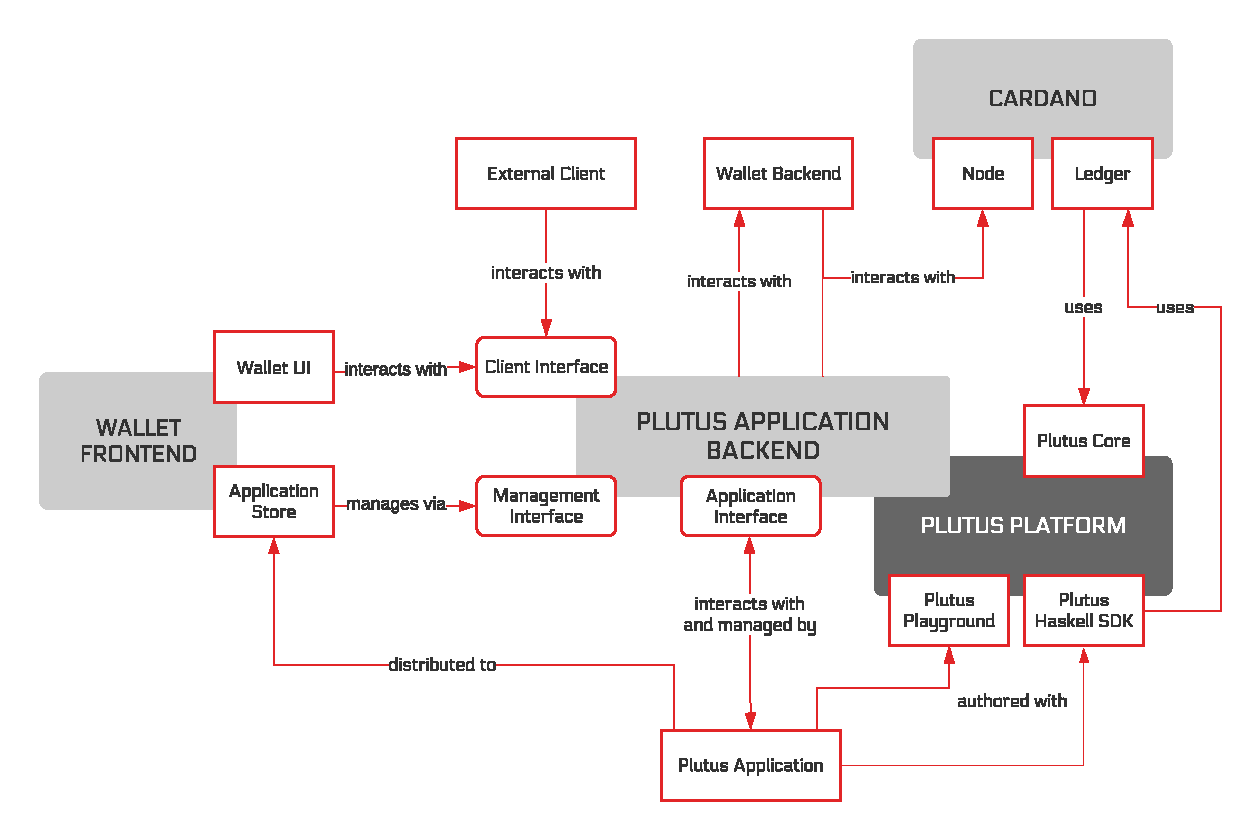
\includegraphics[width=\textwidth]{paf-architecture.pdf}
  \caption{Architecture of the \gls{paf}}
  \label{fig:paf-architecture}
\end{figure}

\subsection{Requirements}
\begin{requirement}[Backups]
\label{req:app-backups}
\Glspl{app} need to be easy to back up, if they are to be used in production.
\end{requirement}

\begin{requirement}[Monitoring]
\label{req:app-monitoring}
\Glspl{app} need to be easy to monitor, if they are to be used in production.
\end{requirement}

\begin{requirement}[Synchronization]
\label{req:app-synch}
It should be possible to synchronize the state of an \gls{app} between instances on multiple machines, e.g. a mobile and a desktop instance.
This is quite important for consumer-type users.
\end{requirement}

\begin{requirement}[Reproducibility]
\label{req:app-reproducibility}
\Gls{app} behaviour should be reliable and reproducible on different environments and devices.
For example, \glspl{app-inst} that have had their state synchronized (\cref{req:app-synch}) should behave identically.
\end{requirement}

\begin{requirement}[Distribution]
\label{req:app-dist}
\Glspl{app} need to be distributed to users somehow.
Different users may have different needs here, for example:
\begin{itemize}
\item A consumer user may want to download an \gls{app} from a centrally managed ``app store'' in their \gls{wallet-frontend}.
\item A business user may want to download a native application via their usual package manager, or directly from the author.
\end{itemize}
\end{requirement}

\begin{requirement}[Flexible, self-describing application endpoints]
\label{req:app-client-interfaces}
\Glspl{app} will want to expose endpoints to users which trigger the functionality of the application.
These need to be accessible to both server-side headless consumers, and also to graphical \glspl{wallet-frontend} which mediate interaction with end-users.

Ideally, these endpoints would be \emph{self-describing} so that we can have at least basic generic interfaces in e.g. a \gls{wallet-frontend}.
\end{requirement}

\begin{requirement}[Chain data access]
\label{req:app-chain-data}
\Glspl{app} need to access some historical data about the chain.
In particular, due to \cref{req:ledger-utxo-size} the \glspl{datum} for \glspl{script-output} are not stored in the \gls{utxo} set, but rather in the transaction that creates the output.
\Glspl{app} will need to know about these \glspl{datum}, so we must provide some way of tracking this information from the chain and making it available.

\todompj{Should link to wherever we discuss the whole issue with storing datums in detail.}
\end{requirement}

\begin{requirement}[Rollback resistance]
\label{req:app-rollback}
Rollbacks can cause serious problems for agents (not just applications) trying to take conditional actions.
It would be nice if we could mitigate these for \glspl{app}, but that may not always be possible.

Here are two scenarios we might care about.

\paragraph{Incoherent choice}
\label{para:incoherent-choice}
Suppose that Alice promises to send 10 \gls{ada} to Bob, provided that Bob sends 20 \gls{ada} to Carol (perhaps Alice is holding Bob's collateral for a loan from Carol, which Bob is now repaying).
The following events occur:
\begin{enumerate}
\item Bob pays 20 \gls{ada} to Carol in transaction T1.
\item Alice observes T1, and proceeds to pay 10 \gls{ada} to Bob in transaction T2.
\item A rollback occurs. After the rollback, T1 and T2 go back into the mempool, but T1 is now invalid.
\item T2 alone is reapplied.
\end{enumerate}

As a result, Alice ends up making the payment to Bob without Bob paying Carol, so Bob gets away with all the money!
Alice ends up committed to an action that she would only have chosen to do the old history of the chain, and which she would not have chosen to do the new history.

\paragraph{Incomplete reapplication}
\label{para:incomplete-reapplication}
Suppose as a variant of the previous scenario that Alice promises to send 10 \gls{ada} to both Bob and Carol, provided that some off-chain event happens.
The following events occur:
\begin{enumerate}
\item The off-chain event occurs.
\item Alice pays 10 \gls{ada} to Bob in transaction T1.
\item Alice pays 10 \gls{ada} to Carol in transaction T2.
\item A rollback occurs. After the rollback, T1 and T2 go back into the mempool, but T1 is now invalid.
\item T2 alone is reapplied.
\end{enumerate}

As a result, Alice ends up only paying Carol and not Bob.
Alice ends up \emph{partially} taking an action that she still wants to take, and would need to reconstruct the missing parts to get back to the state she wants to be in.
\end{requirement}

\begin{requirement}[Testing and emulation]
\label{req:app-emulation}
Users need to be able to test their \glspl{app} in an environment that mirrors the real one as closely as possible.
However, the real environment is very complex, featuring a multi-agent, distributed system with a number of tricky behaviours: network issues, rollbacks etc.

It is therefore desirable to provide some kind of emulated testing harness which users can use to test their \glspl{app} locally, but which allows control and simulation of real issues.

Moreover, this is important for us during development, as it allows us to mock up the system that we expect without having to wait for other components to be ready.
\end{requirement}

\subsection{Lifecycle of a \glsentrytext{app}}

The lifecycle of a \gls{app} is as follows:

\begin{itemize}
\item
  \Glspl{app} are authored and compiled with the \gls{plutus-sdk} using the \gls{app-api} for interacting with other components.
\item
  \Glspl{app} are distributed via some means to be decided, but manually in the interim.
\item
  \Glspl{app} are installed into an instance of the \gls{pab}. The \gls{pab} just knows about the compiled \gls{app-exe} provided by the \gls{app}.
\item
  A \gls{app} can be instantiated into a \gls{app-inst} by running the \gls{app-exe} and providing any parameters that it needs.
  There can be multiple \glspl{app-inst} per \gls{app}, and they are managed by the \gls{pab}.
\item
  The \gls{pab} manages and handles the requirements of the \gls{app-inst} throughout its lifecycle, including interaction with external clients such as \glspl{wallet-frontend}.
\end{itemize}

The major component here is the \gls{pab}.

\subsection{The \glsentrylong{pab}}
\label{sec:pab}

\fbox{
\begin{minipage}{\textwidth}
WARNING: this component is under heavy development, so this will likely evolve and may not represent the current state of things.
\end{minipage}
}
\medskip

A key component of the \gls{paf} is the \glsfirst{pab}.
This is a backend service (like the \gls{wallet-backend}) that intermediates between \glspl{app}, the \gls{node}, the \gls{wallet-backend}, and users (including the \gls{wallet-frontend}).

The \gls{pab} will be run in similar contexts to the wallet backed, e.g. backing a graphical user wallet (e.g. \gls{daedalus}), or on a server that runs \glspl{app} as part of a larger system.

The purpose of the \gls{pab} is to:
\todompj{Do this in prose? Also all the provisions here should be expanded and moved to requirements}
\begin{itemize}
\item Provide a standardized environment for \glspl{app} to run in (\cref{req:app-reproducibility,req:app-monitoring})
\item Provide disciplined state management (\cref{req:app-backups,req:app-synch,req:app-rollback})
\item Present discoverable interfaces to the external clients (\cref{req:app-client-interfaces})
\item Track information from the chain for use by contracts (\cref{req:app-chain-data})
\item Work in an emulated environment (\cref{req:app-emulation})
\end{itemize}

The \gls{pab} is a series of components which produce/consume events, and a message bus.

Some of the components have additional complexity, e.g. the application management component needs to manage the state of \glspl{app-inst}.

\subsubsection{Node client}
The \gls{pab} needs to talk to the \gls{node}, primarily because it needs to populate the \gls{chain-index}, but it may also need to do some things that appear to be the \gls{wallet-backend}'s job (e.g. maintaining pending sets), because we can't guarantee that the \gls{wallet-backend}'s view of the world will match our own (since each is independently talking to the \gls{node}).

\subsubsection{\Glsentrytext{wallet-backend} client}

The \gls{pab} needs to talk to the \gls{wallet-backend} for a number of things:
\begin{itemize}
\item Coin selection/transaction balancing
\item Transaction signing and submission
\item Address creation
\end{itemize}

You might think that since the \gls{pab} has a node client itself, it could do its own transaction submission, and only rely on the \gls{wallet-backend} for signing.
However, transactions made by the \gls{pab} will likely use outputs ``owned'' by the \gls{wallet-backend} (e.g. those selected by coin selection from the user's outputs).
Hence it is important that the \gls{wallet-backend} knows about such outputs, so that it does not attempt to spend them somewhere else.

\subsubsection{Event system}

The \gls{pab} needs to handle incoming events from a number of sources concurrently, so we need some kind of message bus.
In addition, the persistence story for \glspl{app-inst} involves persisting their incoming events, so this is a good fit.

We are currently using an event-sourced architecture here.
We hope that this will make backups and synchronization easier (\cref{req:app-backups,req:app-synch}).

\subsubsection{Application management}

\Gls{app-inst} need to be managed, created, destroyed, fed with events, etc.

\begin{itemize}
\item Create \glspl{app-inst}
\item Instantiate and run \glspl{app-exe} in a sandbox
\item Handle communication with the \gls{app-exe}
\item Handle own message queue (``mailbox'') for each \gls{app-inst}
\item Manage/dump/load \glspl{app-inst}
\item Create/destroy \glspl{app-inst}
\item Handle rollbacks
\end{itemize}

\subsubsection{\Glsentrytext{chain-index}}

Applications need to access \glspl{datum} for outputs (see \cref{req:app-chain-data}), so we need some kind of system that monitors the chain and records (at least) the \glspl{datum}.

\subsubsection{Client interface}

For external clients (other programs), including graphical \glspl{wallet-frontend} to talk to.
Should expose some of the application endpoints and \gls{app-inst} management functionality.

\subsubsection{Logging and monitoring}

To satisfy \cref{req:app-monitoring}.

\subsection{Emulators}

In order to satisfy \cref{req:app-emulation}, we need to write emulators for quite a number of components.

At present, we have (or expect to have) emulators for:
\begin{itemize}
\item
  The \gls{node} using our ledger extensions.
  In the long run we should be able to use the real Goguen \gls{node}.
\item
  The parts of the \gls{wallet-backend} that we need.
  In the long run we \emph{might} be able to use the real \gls{wallet-backend}.
\item
  Basic \gls{wallet-frontend} functionality, such as displaying balances and interacting with \glspl{app-inst}.
  In the long run we \emph{might} be able to use the real \gls{wallet-frontend}, but this seems unlikely as it is quite heavyweight.
  Having our own component here has the advantage that we can reuse it in the \gls{plutus-playground}.
\end{itemize}

We also need libraries to bind all of these into an overall, multi-agent simulation, and to allow users to write tests that exercise particular series of events in this simulation.

\subsection{The \glsentrytext{plutus-playground}}
\label{sec:plutus-playground}

The \gls{plutus-playground} provides a Web environment for getting started with the \gls{plutus-platform}.

The authoring experience in the \gls{plutus-playground} is fairly limited (one file only), but it has the best support for specifying ad-hoc scenarios and visualizing the results.

Over time we hope to unify the experiences of working locally and working in the \gls{plutus-playground}, by:
\begin{itemize}
\item Improving the authoring experience in the \gls{plutus-playground} (multiple files etc.)
\item Improving the visualization experience locally (sharing components with the \gls{plutus-playground})
\item Allowing distribution of simple \glspl{app} directly from the \gls{plutus-playground}.
\end{itemize}

\subsection{Application design}

\todompj{Talk about state machines and our ideas for handling rollbacks.}

\end{document}

\section{Related work}

\paragraph{Ethereum.}

Ethereum's ERC token standards~\cite{erc20,erc721} are one of the better known multi-asset
implementations. They are a non-native implementation and so come with a set of drawbacks,
such as having to implement ledger functionality (such as asset transfers) using smart contracts, rather
than using the underlying ledger.

Augmenting the Ethereum ledger with functionality similar to that of the model
we present here would likely be possible. Additionally, access to global
contract state would make it easier to define forging policies that care about
global information, such as the total supply of an asset.

\paragraph{Waves.}

Waves~\cite{waves} is an account-based multi-asset ledger, supporting its own smart contract
language. In Waves, both accounts and assets themselves can
be associated with contracts. In both cases, the association is made by
adding the associated script
to the account state (or the state of the account containing the asset).
A script associated with an asset imposes conditions on the use of this asset,
including minting and burning restrictions, as well as transfer restrictions.

\paragraph{Stellar.}

Stellar~\cite{stellar} is an account-based native multi-asset system geared towards tracking
real-world item ownership via associated blockchain tokens.
Stellar is optimised to allow a token issuer to maintain a level of control over
the use of their token even once it changes hands. The Stellar ledger also features
a distributed exchange listing, which is used to
facilitate matching (by price) exchanges between different tokens.

\paragraph{Zilliqa.}

Zilliqa
is an account-based platform with an approach to smart contract implementation
similar to that of Ethereum~\cite{scilla-arxiv}.
The Zilliqa fungible and non-fungible tokens are
designed in a way that mimics the ERC-20 and ERC-721 tokens, respectively.
While this system is designed to be statically analysable, it does not offer new solutions to
the problem of dependency on the global state.

\paragraph{DAML.}

DAML~\cite{daml} is a smart contract language designed to be used on the DAML ledger model.
The DAML ledger model does not support keeping records of asset ownership, but instead,
only stores current contract states in the following way:
a valid transaction interacting with a contract results in the creation of new
contracts that are the next
steps of the original contract, and removal of the original contract from the ledger.

Only the contracts with which a transaction
interacts are relevant to validating it, which is similar to our approach
of validation without global context.
Although this system does not have built-in multi-asset support (or any
ledger-level accounting),
the transfer of any type of asset can be represented on the ledger via contracts.
Due to the design of the system to operate entirely by listing contracts on the ledger,
each
action, including accepting funds transferred by a contract, requires consent. This
is another significant way
in which this model is different from ours.

%\todompj{This doesn't actually say anything about multi-asset stuff?}

\paragraph{Bitcoin.}

Bitcoin popularised \UTXO\ ledgers, but has neither native nor non-native
multi-asset support on the main chain.
The Bitcoin ledger model does not appear to have the accounting infrastructure
or sufficiently expressive
smart contracts for implementing multi-asset support in a generic way.
There have been several layer-two approaches to implementing custom Bitcoin assets.
Because each mined Bitcoin is unique, a particular
Bitcoin can represent a specific custom asset, as is done in~\cite{coloredcoins}.
A more sophisticated accounting strategy is implemented in another layer-two
custom asset approach~\cite{nick2020liquid}.
There have also been attempts to implement custom tokens using Lightning network
channels~\cite{lntokens}.

\paragraph{Tezos.}

Tezos~\cite{tezos} is an account-based platform with its own smart contract language.
It has been used to implement an ERC-20-like fungible token standard (FA1.2),
with a unified token standard in the works (see~\cite{tezosMA}).
The custom tokens for both multi-asset standards are non-native, and thus have shortcomings
similar to those of Ethereum token standards.

%\todompj{This is very vague.}

\paragraph{Nervos CKB.}

Nervos CKB~\cite{nervos} is a \UTXO{}-inspired platform that operates on a broader notion of a Cell,
rather than the usual output balance amount and address, as the value stored in
an entry. A Cell entry can contain any type of data,
including a native currency balance, or any type of code.
This platform comes with a Turing-complete scripting language that can be used to define custom
native tokens. There is, however, no dedicated accounting infrastructure to handle
trading custom assets in a similar way as the base currency type.

\section{Discussion}
\label{sec:discussion}

\subsection{General observations}
\subsubsection{Asset registries and distributed exchanges.}

The most obvious way to manage custom assets might be to add some kind of global \emph{asset registry}, which associates a new asset group with its policy.
Once we have an asset registry, this becomes a natural place to put other kinds of infrastructure that rely on global state associated with assets, such as decentralised exchanges.

However, our system provides us with a way to associate forging policies and the assets controlled by them \emph{without} any global state. This simplifies the ledger implementation in the concurrent and distributed environment of a blockchain.
Introducing global state into our model would result in disrupted synchronisation (on which \cite{chakravarty2020hydra} relies to great effect to implement fast, optimistic settlement), as well as slow and costly state updates at the time of asset registration.
Hence, on balance we think it is better to have a stateless system, even if it relegates  features like decentralised exchanges to be Layer 2 solutions.

% MPJ: I don't think this adds anything

%Similarly, when we think about facilitating the trading custom tokens, we might want to include or facilitate a
%\emph{decentralised exchange} as part of our system.
%However, again such a listing requires global state to track the offers.

%Note that our model allows for a fair and reliable way for users
%to make offers of MA tokens
%for sale or exchange on the ledger. To make such an offer, a user would place
%their tokens in an output locked by a script. This script requires the transaction spending
%this output to \emph{pay} for the token.

%It is possible to implement a decentralised exchange listing or a global
%asset registry in a
%in a way that does not compromise security guarantees of our current model, but
%at the expense of high overhead, complicated validation rules,
%and frequent transaction validation failure.
%All transactions submitted, but not processed, before a registry update would
%necessarily become invalid, which would be a frequent occurence.

%Even with a design of a registry that solves these problems, it does not make
%sense to have either registry be the main
%source of truth in our model, since their functionality must be specified
%elsewhere, i.e. the relevant forging and output scripts.

\subsubsection{Spending policies.}

Some platforms we discussed provide ways to express restrictions on the \emph{transfer} of
tokens, not just on their forging and burning, which we refer to as \textit{spending policies}.
Unlike forging policies, spending polices are not a native part of our system.
We have considered a number of approaches to adding spending policies, but we
have not found a solution that does not put an undue burden on the \emph{users}
of such tokens, both humans and programmatic users such as layer-two protocols
(e.g. Lightning). For example, it would be necessary to ensure that spending
policies are not in conflict with forging or output-locking scripts (any time the asset is spent).

Forging tokens requires a specific action by the user (providing and satisfying a forging policy script), but this action is always taken knowingly by a user who is specifically trying to forge those tokens.
\emph{Spending} tokens is, however, a completely generic operation that works over arbitrary bundles of tokens.
Indeed, a virtue of our system is that custom tokens all look and behave uniformly.
In contrast, spending policies make custom tokens extremely difficult to handle in a generic way, in particular for automated systems.

These arguments do not invalidate the usefulness of spending policies, but instead highlight that
they are not obviously compatible with trading of native assets in a generic way, and an approach that addresses these issues in an ergonomic way is much needed.
This problem is not ours alone: spending policies in other systems we have looked at here (such as Waves),
do not provide universal solutions to the issues we face with spending policies either.

\subsubsection{Viral scripts.}

One way to emulate spending policies in our system is to lock all the tokens with a particular script that ensures
that they \emph{remain} locked by the same script when transferred.
We call such a script a ``viral'' script (since it spreads to any new outputs that are ``infected'' with the token).

This allows the conditions of the script to be enforced on every transaction that uses the tokens, but at significant costs.
In particular such tokens can never be locked by a \emph{different} script, which prevents such tokens from being used in smart contracts, as well as preventing an output from containing tokens from two such viral asset groups (since \emph{both} would require that their validator be applied to the output!).
In some cases, however, this approach is exactly what we want.
For example, in the case of credential tokens, we want
the script locking the credential to permanently allow the issuer access to the credential (in
order to maintain their ability to revoke it).

\subsubsection{Global State.}

There are limitations of our model due to the fact that global information about the ledger is not available to the forging policy script.
Many global state constraints can be accommodated with workarounds (such as in the case of provably unique fresh tokens), but some cannot:
for example, a forging policy that allows a variable amount to be forged in every block depending on the current total supply of assets of another policy.
This is an odd policy to have, but nevertheless, not one that can be defined in our model.

\subsection{Conclusions}

We present a multi-asset ledger model which extends a UTXO-based ledger so that it can support custom fungible and non-fungible tokens.
We do this in a way that does not require smart contract functionality.
We add a small language with the ability to express exactly the logic we need for a particular set of usecases.
Our \UTXOma{} ledger together with this language allows us to use custom assets to support a wide variety of usecases, even those that are not normally based on ``assets'', while still remaining deterministic, high-assurance, and analysable.

Our design has a number of limitations, some of which have acceptable workarounds, and some that do not.
In particular, access to global state in a general way cannot be supported, and spending policies are not easy to implement.
It is also not possible to explicitly restrict payment to an address.
We consider these worthy directions for future improvements to our model.


% MPJ: This doesn't seem relevant? Nothing to do with multi-asset really
%\paragraph{Transfer restrictions imposed by the recepient.}
%
%In our system, we do not provide a default way to restrict payment to
%an address. We have discussed two platforms where this is possible, Nervos and
%DAML, both of which have fundamentally different designs that compromise other
%features we require in ours. These types of restriction policies
%are closely related to and suffer from many of the same problems as
%spending policies, such as high overhead, clashing constraints with sequetial or
%parallel contracts, and the possibility of circumvention.

% Doesn't tell anything new -=chak
%\section{Conclusion}
%
%We have presented \UTXOma{}, a \UTXO{} ledger model with native, lightweight, stateless mulitasset support.
%\UTXOma{} supports a wide range of key use cases, including fungible and non-fungible tokens.
%
%Moreover, we show that a simple scripting model is adequate to implement a variety of both useful forging policies and output-locking scripts.
%Using these together we are able to realise a wide variety of applications.

% MPJ: I think we can get away with a simpler conclusion

%With our two-level token classification structure, we are able to both
%\begin{itemize}
%  \item infer the fungibility relation directly by looking at the names and IDs of
%  token classes, without executing code
%  \item retain the ability to impose fungibility constraints, as tokens under a single
%  policy are minted and burned, by rejecting attempts to forge tokens that do not satisfy them
%\end{itemize}

%As promised, we gave examples of clauses that a language would need in order to express
%a number of interesting and realistic use cases.
%Defining language clauses in this way, however, is one step away from hard-coding scripts into
%rules about processing transactions, and frequently requires updating them
%every time we encounter a new use case.

%There are many advantages to making this system more expressive, with a fully
%formed scripting language. The approach we present here, however, gives use the opportunity to highlight
%just how versatile and intuitive our MA structure us due to being native and
%represented by the two-level map we described. Even with a minimally expressive
%smart contract language (only checking multi-signatures), we can already allow users to
%define asset policies governing the forging of custom tokens.


\bibliographystyle{splncs04}
\bibliography{utxoma}

\end{document}
